
% last updated in April 2002 by Antje Endemann
% Based on CVPR 07 and LNCS, with modifications by DAF, AZ and elle, 2008 and AA, 2010, and CC, 2011; TT, 2014; AAS, 2016

\documentclass[runningheads]{llncs}
\usepackage{graphicx}
\usepackage{amsmath,amssymb} % define this before the line numbering.
\usepackage{ruler}
\usepackage{color}
\usepackage[width=122mm,left=12mm,paperwidth=146mm,height=193mm,top=12mm,paperheight=217mm]{geometry}
\usepackage{url}
\usepackage{hyperref}
\usepackage{tabularx}


\begin{document}
% \renewcommand\thelinenumber{\color[rgb]{0.2,0.5,0.8}\normalfont\sffamily\scriptsize\arabic{linenumber}\color[rgb]{0,0,0}}
% \renewcommand\makeLineNumber {\hss\thelinenumber\ \hspace{6mm} \rlap{\hskip\textwidth\ \hspace{6.5mm}\thelinenumber}}
% \linenumbers
\pagestyle{headings}
\mainmatter
\def\ECCV16SubNumber{***}
\title{DD2424 Project - character-level text classification with different RNN architectures}

\maketitle

%The final report should include the following sections:

\begin{abstract}
% • Abstract: Where you give an overview of the task and the findings
% of your work in a nutshell.

\dots
\keywords{We would like to encourage you to list your keywords within
the abstract section}
\end{abstract}


\section{Introduction}

% • Introduction/Problem formulation: Motivate the problem you
% are trying to solve, attempt to make an intuitive description of the
% problem and also formally define the problem. (1-2 pages including
% title, authors and abstract)

We are looking at a text classification problem with short text and character-level classification. We will be using character-level classification. This means that the network processes the input one character at a time. Each character results in an output consisting of the probabilities for each letter for the next character. If we have a 58-character alphabet, the hidden state will consist of the probability of each of those 58 characters for the next letter in the sequence. So for each character, one such prediction is produced, as well as a hidden state, which is fed into the next step.

Short-text classification is hard in that there is less information to go off with little to no grammar or syntax. Some applications of short-text classification include search queries and information retrieval, mapping a product name to its associated product, the classification of titles, questions, sentences, and short messages.

The texts we are looking at are names of cities, and the classes are the names of the country the city belongs to. To begin with, we used the world-cities data set. We later abandoned it for geonames, because it has more samples. There are circa 240 categories (countries) in the data sets, but we will limit the number of categories so as not to make the categories too unevenly distributed (ie remove countries with too few cities in the data set).

The inspiration for the project is \href{https://github.com/spro/practical-pytorch/blob/master/char-rnn-classification/char-rnn-classification.ipynb}{a tutorial}
 in which a recurrent network is used to classify names as belonging to certain nationalities, using the Python framework \textit{Pytorch}. To start with, the model of that tutorial is to be replicated, then additional architectures will be implemented and compared. Questions we ask ourselves include: to what degree would a deeper network help in this problem? What sort of architectures are good in this application? Would an LSTM-layer in the recurrent network give better results? 

To measure the success of the text classification, we will look at the precision, recall and f1-score of each category in the data set. This because it gives a more nuancued evaluation than accuracy, seeing as how the data set used is heavily skewed. Furthermore, we will visualize the results with a confusion matrix.


\section{Background}

% • Background: summarize a few notable approaches/papers tackling
% the same problem. The selection should cover different possible tech-
% niques that can be (have been) used for the same task with success.
% Also, it is good to mention other recognition/synthesis tasks that use
% the same deep learning technique as yours. (1-2 pages)


\section{Approach}
% • Approach: Describe the final approach you are take for this problem.
% For instance, here you would describe the details of the network’s
% architecture. What training parameters and techniques you have used.
% The computational complexity of your model. And similar questions.
% To help explain your approach please make figures to accompany your
% text description. (1-3 pages)

\section{Experiments}

The first experiment was simply taking the model from the tutorial and running it on the first data set we had decided upon, the world-cities data set. 


\begin{figure}[h!]
	\centering
    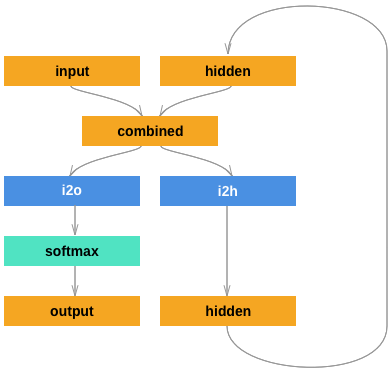
\includegraphics[width=.5\textwidth]{../plots/tutorial_model.png}
	\caption{ Model from the text classification tutorial.}
	\label{fig:model_tutorial}
\end{figure}

The model in the tutorial is seen in figure \ref{fig:model_tutorial}, where i2o and i2h are simple linear layers that do a $y=Wx + b$ type calculation. Softmax is used to assign the different categories probabilities - it is a good way to represent a categorical distribution in a multi-class problem such as this one.
The criterion for loss that is used is negative log-likelihood loss.
The optimizer that is used is stochastic gradient descent. No momentum is used.
The \textit{combined} layer simply concatenates the input vector and hidden vector.

The data preprocessing was simple: the data was converted to ASCII-characters and the data was filtered to only have countries with at least 100 cities in the data set. This because the initial distribution was a bit too uneven, as seen in figure \ref{fig:world_cities}, with many countries having very few cities, some even just 1 or 2. What remained was 18684 data points.

\begin{figure}[h!]
	\centering
	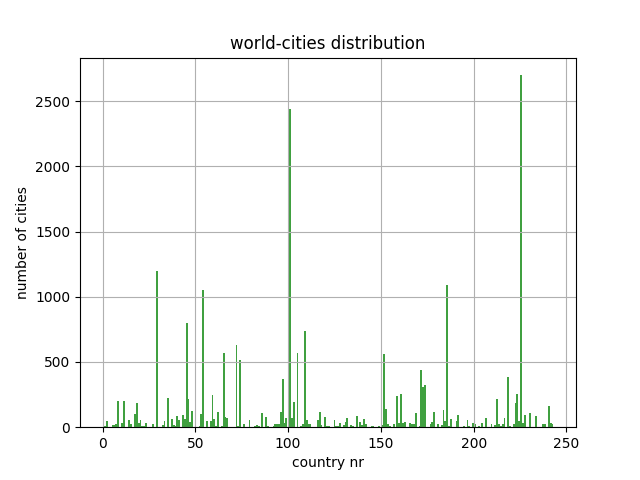
\includegraphics[width=.5\textwidth]{../plots/dist.png}	
	\caption{ World-cities distribution.}
	\label{fig:world_cities}
\end{figure}

The training was done in a similar way as in the tutorial, with random sampling with replacement from the data set. The final confusion matrix looked is presented in figure \ref{fig:conf_init},
and the final average f1 score (averaged over all the categories) was 0.3. The test accuracy was 31 percent.

\begin{figure}[h!]
	\centering
        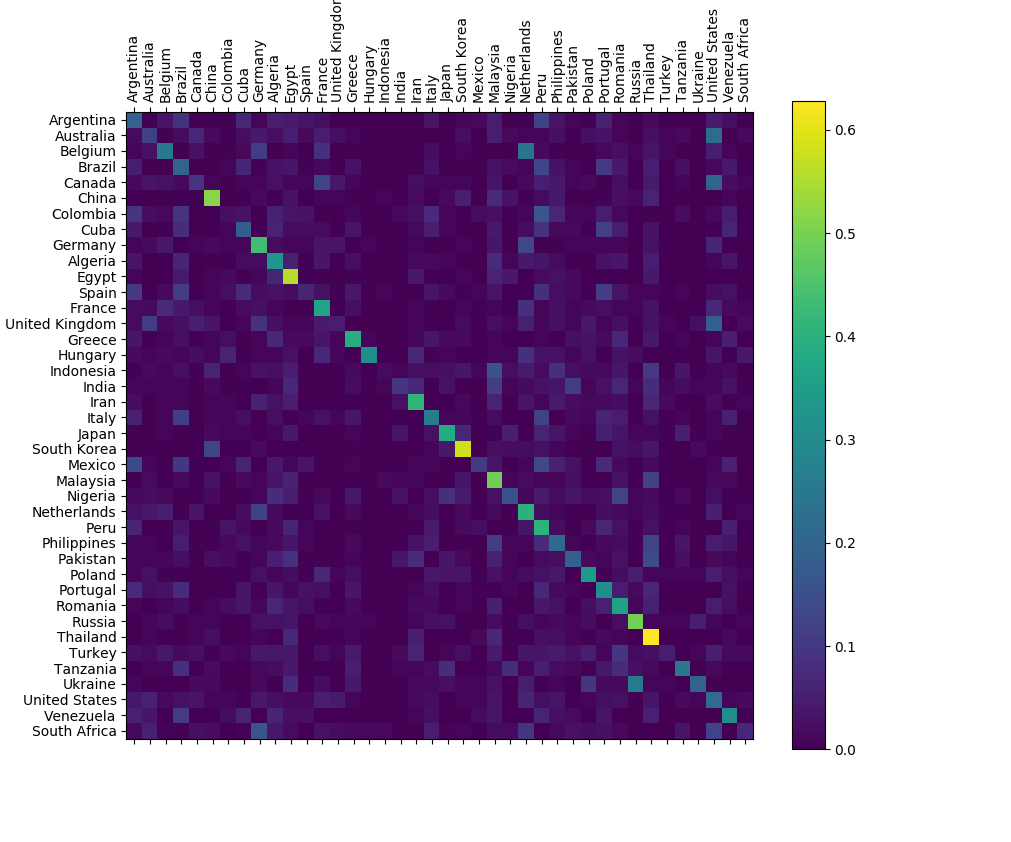
\includegraphics[width=.5\textwidth]{../plots/confusion_matrix_initial.png}
	\caption{ Confusion matrix of first RNN model.}
	\label{fig:conf_init}
\end{figure}


While it is true that the model has a pretty good accuracy for some of the categories, it is still performing pretty unevenly for the categories. As seen in the figure, it is moderately good at classifying countries like Thailand and Korea, but not very good at classfiying countries like Colombia or Indonesia (indeed it seems to never predict them). We do not see a clear pattern from the class distribution (for example the US is overrepresented in the data set but is not predicted more often than other countries). This is because of how the random sampling is made - first a random category is chosen, then a sample will be taken randomly from that category. Therefore, the number of times we're exposed to samples from different categories will be more or less even.

\subsection{Introducing LSTM and GRU}

We wanted to see if an LSTM-layer could improve the performance of the network. LSTMs are units used in recurrent networks that are composed of several gates - an input gate, output gate and forget gate. The LSTM can choose to "remember" or "forget" inputs from the past. This mechanism allows them to avoid the long-term dependency problem. However, this might not matter in this particular short-text classification problem, since there should not be long-term dependencies.

LSTMs are also supposed to be good against exploding and vanishing gradients, which is a common problem in backpropagation-through-time, the most common learning algorithm for standard recurrent networks.


When we have an LSTM cell in Pytorch, it takes an input, a hidden state and a cell state and it does the following computations

\begin{gather}
	i_t = \sigma(W_{i,i} x_t + b_{i,i} + W_{h,i} h_{t-1} + b_{h,i}) \\
	f_t = \sigma(W_{i,f}x_t + b_{i,f} + W_{h,f}h_{t-1} + b_{h,f}) \\
	g_t = tanh(W_{i,g}x_t + b_{i,g} + W_{h,g}h_{t-1} + b_{h,g}) \\
	o_t = \sigma(W_{i,o}x_t + b_{i,o} + W_{h,o}h_{t-1} + b_{h,o}) \\
	c_t = f_tc_{t-1} + i_tg_t \\
	h_t = o_t tanh(c_t)
\end{gather}

where $h_t$ is the hidden state at time t, $c_t$ is the cell state at time t, $x_t$ is the input, $h_{t-1}$ is the hidden state at the previous time step and $i_t$, $f_t$, $g_t$ and $o_t$ are the input, forget, cell and output gates. \cite{torchdoc}

In other words, the LSTM cell works by applying nonlinear functions to both inputs and internal variables. 
% TODO: write more about LSTMs

 
The first LSTM experiment was simply running the same model as before, but replacing the linear layer for an LSTM layer.
 
\begin{figure}[h!]
	\centering
        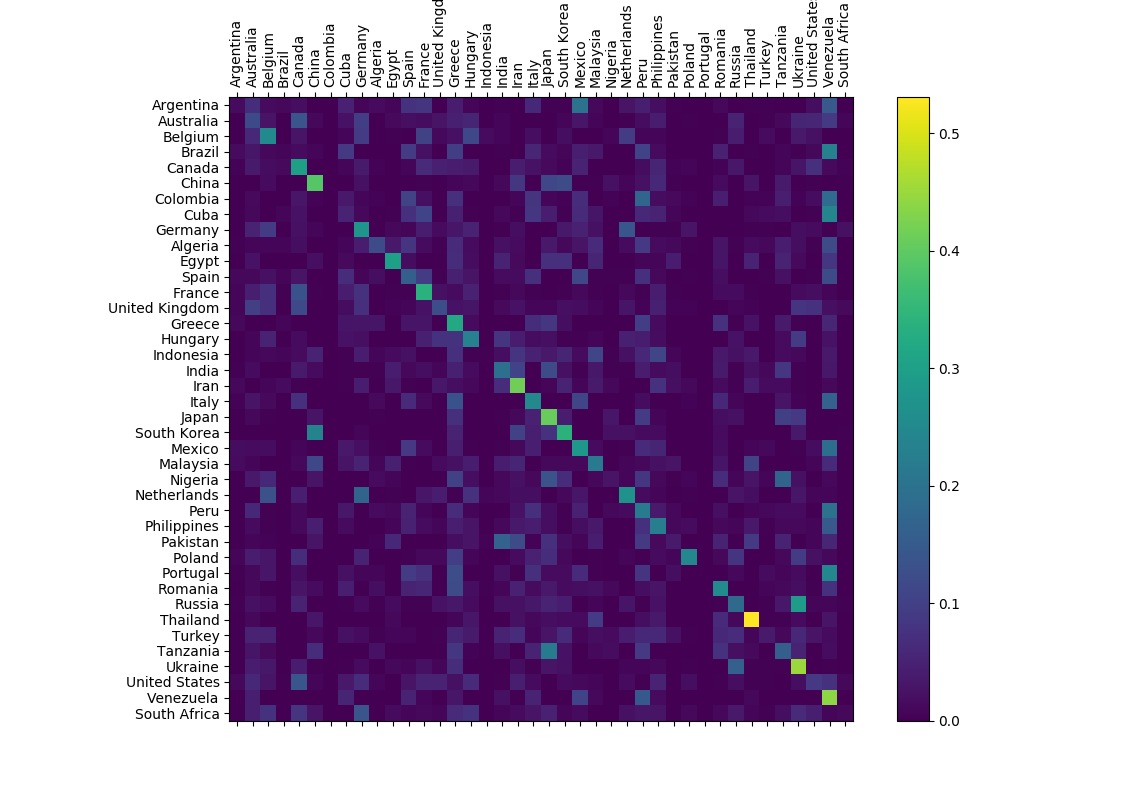
\includegraphics[width=.5\textwidth]{../plots/conf_matrix_initial_LSTM.png}
	\caption{ Confusion matrix of first LSTM model.}
	\label{fig:conf_initial_lstm}
\end{figure}
 
It ended up not performing as well as the standard RNN after having been trained in the same way (same hyper-parameters, same number of epochs). As seen in figure \ref{fig:conf_initial_lstm}, the max accuracy is 0.5 rather than 0.6, and there are more incorrect predictions.
 
Some more iterations of different LSTM architectures were tried.
Things that were changed for each model are laid out in table \ref{tab:LSTMs}, and the results of the models are seen in table \ref{tab:LSTM_models}.

\begin{table}[h!]
    \begin{center}
        \caption{The changes introduced to different models.}
        \label{tab:LSTMs}
        \begin{tabularx}{.9\textwidth}{ | c | c | }
	        \hline
	        \textbf{LSTM model nr} & \textbf{difference introduced} \\ \hline
	        1 & introduced LSTM layer \\ \hline
	        2 & \begin{tabular}[x]{@{}c@{}} did combined input and \\ hidden (as in the original RNN)\end{tabular} \\ \hline
	        3 &  \begin{tabular}[x]{@{}c@{}} used a new data set called geonames,\\ that had more training samples\end{tabular} \\ \hline
	        4 & \begin{tabular}[x]{@{}c@{}} the previous model ran on all \\ countries in geonames that had more than 100 cities. \\ here the data was filtered more, and only \\ countries with more than 300 cities were used \end{tabular} \\ \hline
	        5 & tried not having class weights, to see if it actually helped \\ \hline
	        6 & used two LSTM layers \\ \hline
	        7 & \begin{tabular}[x]{@{}c@{}} instead of randomly sampling \\ with replacement, training consists of running \\ through the entire data set consisting of 81526 samples. \\ it was trained for 10 epochs \end{tabular} \\ \hline
	        8 & \begin{tabular}[x]{@{}c@{}} ran the model for 20 epochs. \\ checked validation error after every epoch. \\ also introduced shuffling of the data \\ before every epoch \end{tabular} \\ \hline
        \end{tabularx}      
        \end{center}
\end{table}
 

\begin{table}[h!]
    \begin{center}
        \caption{Results of the LSTM models.}
        \label{tab:LSTM_models}
        \begin{tabularx}{.5\textwidth}{ | c | c | c |}
			\textbf{model nr} & \textbf{average f1} & \textbf{test accuracy} \\
			1 & 0.18 & 21.6 \\
			2 & 0.2  & 21.9 \\
			3 & 0.04 & 7.5 \\
			4 & 0.14 & 17 \\
			5 & 0.2  & 17.2 \\
			6 & 0.1  & 12.8 \\
			7 & 0.23 & 27 \\
			8 & 0.3  & 38 \\
         \end{tabularx}  
    \end{center}
\end{table}

       
All LSTM models performed worse than the original RNN, up until model 8. Introducing the data set with more data points did not immediately lead to better results. This because there was an even bigger difference between classes (see figure \ref{fig:geonames}). 

\begin{figure}[h!]
	\centering
	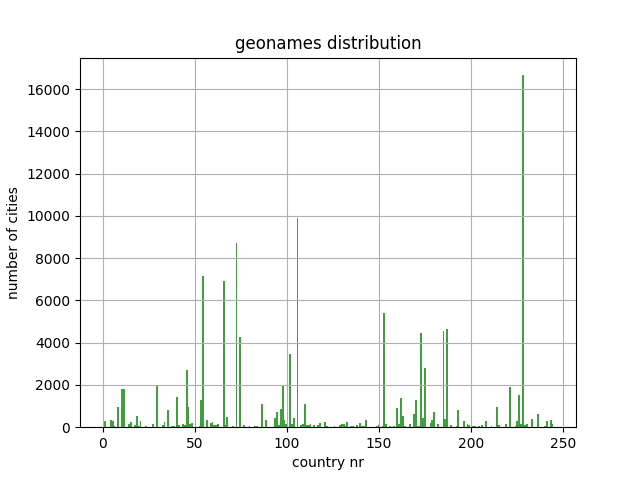
\includegraphics[width=.5\linewidth]{../plots/geonames_set.png}
	\caption{ Geonames data set distribution.}
	\label{fig:geonames}
\end{figure}

This seemed to indicate that the data set needed to be filtered more, so all countries with less than 300 cities were removed.

After filtering the data more, the results were a bit better. However, the accuracy was still pretty low. This because the random sampling of data points meant all categories received the same attention, which was not good in terms of accuracy because some categories were indeed heavily overrepresented in the data set but not in the predictions of the model.
Likewise, the model did not immediately perform better with two LSTM layers rather than one. It turns out that it simply needed to run for more epochs to account for the bigger data set and the bigger model. Indeed, model 8 performed best so far because it was run for more epochs.
 
After this, a GRU model was implemented and tested. It was run in the same way as LSTM model 8. And out of curiosity, a similar standard two-layer RNN was run in the same way. The result of this comparison is seen in table \ref{tab:GRU_LSTM_RNN_comp}.


\begin{table}[h!]
    \begin{center}
        \caption{Comparing the LSTM model with a similar model with GRU layers and one with linear layers.}
        \label{tab:GRU_LSTM_RNN_comp}
		\begin{tabularx}{.8\textwidth}{ | c | c | c |}
			\textbf{model description} & \textbf{average f1} & \textbf{test accuracy} \\
			LSTM model 8 & 0.3 & 38 \\
			similar GRU model & 0.32  & 42 \\
			similar standard RNN model & 0.09 & 12 \\
		\end{tabularx}  
    \end{center}
\end{table}

The GRU performed similar to the LSTM, just slightly better. However, it trained markedly faster. Meanwhile, the simpler RNN did not perform well, as it started suffering from exploding gradients. In its predictions, it exclusively predicted countries that are overrepresented in the data set. 

\section{Results}
\section{Conclusions}

% • Experiments/Results/Conclusions: In this section, you should
% present the results you achieved with various experiments. The re-
% sults can be presented in tables, plots, etc. Explain what conclusions
% you can draw from these set of experiments? The set of experiments
% and results reported here should justify some of the design choices
% described in the previous sections. (3-6 pages)

As \cite{Alpher04} said.

% • References: It is extremely important to make sure all the content
% from other sources and the ideas that you build on are properly cited.


% Both positive and negative results should be reported. A discussion re-
% garding why certain techniques worked better than the others is necessary.
% Students are also encouraged to take initiatives in trying out new techniques,
% beyond those discussed at the lectures.
% The stated number of pages above is a guideline, one can go beyond that or
% slightly below. The whole report should be between 7-14 pages.


\bibliographystyle{splncs}
\bibliography{egbib}
\end{document}
